\kapitola{Literární rešerše}
\sekce {Problematika detekce duplicit v~datech}
\todo{Základní pojmy, metriky, typy algoritmů, problémy s~kvalitou dataaasdasdaa}
Data v rámci různých ekosystémů jsou ukládáná v různých formách. Liší se ve struktuře, pojmenování atributů a hlavně ve způsobu využívání unikátních identifikátorů datových entit. Ve chvíli kdy se pokoušíme data z takových různých zdrojů agregovat například do centrální databáze, vzniká problém. Tím je rozhodnout, které záznamy (entity) jsou unikátní, a které jsou například duplikované z toho důvodu, že prostředí ze kterých jsou získána mají odlišnou strukturu a nelze snadno rozhodnout o tom, zda je daná entita shodná s entitou z jiného zdroje na základě jejího identifikátoru.

V literatuře se objevuje několik termínů, které označují procesy pro nalezení duplicit a vypořádání se s nimi. Přestože se některé z nich používají zaměnitelně, některé zdroje popisují procesy rozdílně. Zde je stručný přehled.

\begin{itemize}
    \item \textit{Data matching} je obecný pojem označující různé techniky pro porovnávání a rozpoznávání duplicit mezi různými zdroji dat.\cite{christen_data_2012}
    \item \textit{Entity resolution} zahrnuje proces nalezení shodných entit s důrazem na spojení těchto entit do jedné entity. \cite{quantexa_what_2024}
    \item \textit{Record linkage} zahrnuje proces nalezení a propojení entit. Narozdíl od \textit{entity resolution} je však nespojuje do jedné entity, ale vytváří se např. propojovací tabulky. \cite{stepanenko_what_2024}
\end{itemize}

Nicméně, tyto rozdíly se objevují pouze v některých zdrojích a to svědčí o tom, že většina těchto a další podobných termínů vznikla v různých oborech a v rámci řešení různých problémů a proto není příliš důležité věnovat se označení procesu, ale spíš procesu jako takovému a krokům, které vedou k nalezení duplicit.\cite{christen_data_2012}

V této práci bude používán termín  \textit{data matching}, převážně z toho důvodu, že podle Google Trends \cite{google_trends_google_2024}, je celosvětově za posledních 5 let termín \textit{data matching} relativně vyhledávanější než ostatní alternativní termíny. Viz. obr. \ref{fig:google-trends}.

\begin{figure}[htb]
    \centering
    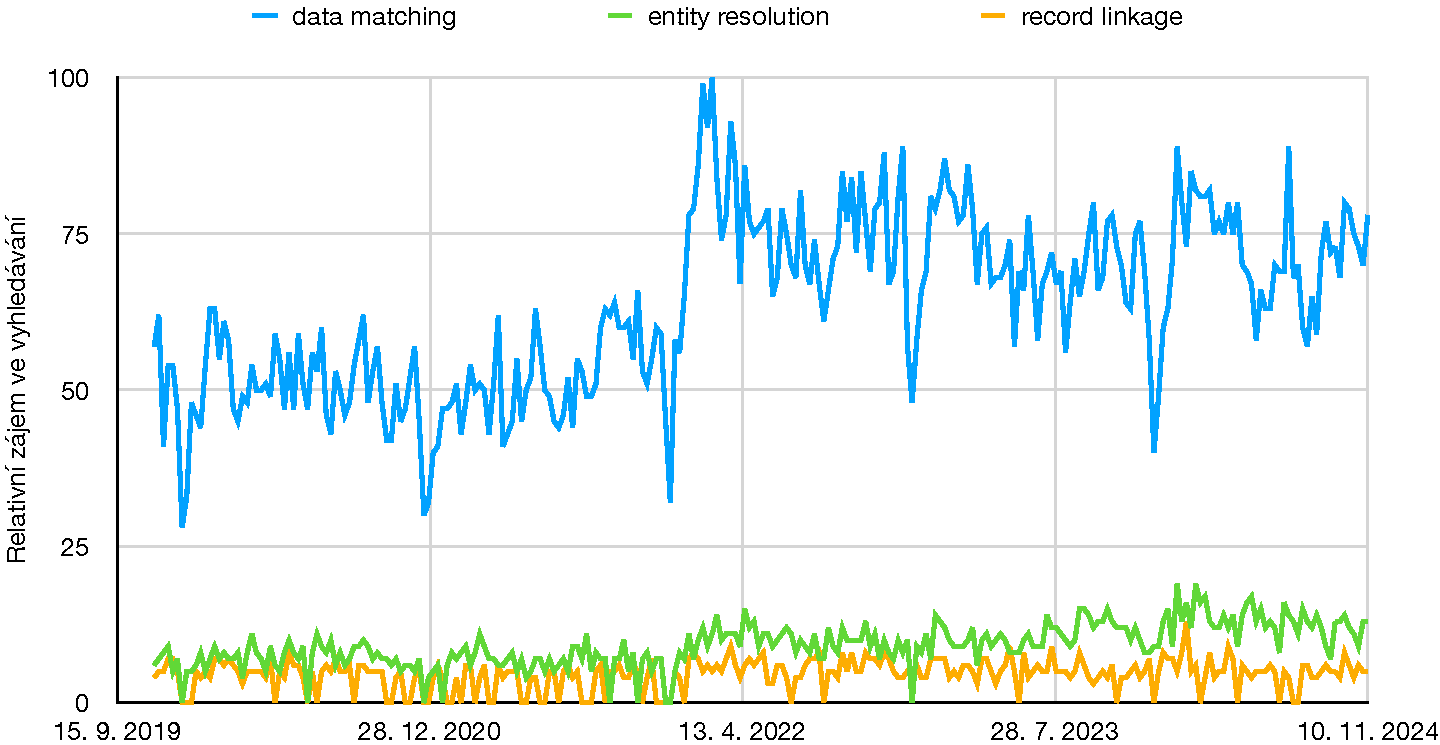
\includegraphics[scale=0.6]{images/google-trends.pdf}
    \caption{Zájem o termíny "data matching", "entity resolution" a "record linkage".\newline
             \textit{Zdroj}: \cite{google_trends_google_2024}}
    \label{fig:google-trends}
\end{figure}
\pagebreak

Příkladem kdy k takovému problému nedojde může být případ z prostředí České republiky a předpokládejme, že jde o data čistě občanů České republiky, kdy máme první datový zdroj s pacienty ordinace a druhý zdroj je databáze klientů zdravotní pojišťovny. V tomto případě lze snadno rozpoznat dané entity (osoby) na základě rodného čísla, které se u záznamů v těcho zdrojích pravděpodobně nachází. V tomto případě můžeme následně data zagregovat a dále s nimi pracovat.

\sekce {Přístupy k~rozpoznání duplicitních entit}
Detekce duplicit bez využití strojového učení zahrnuje například algoritmus pro výběr párů Sorted-Neighborhood-Method (SNM). Je možné provést porovnání všech možných kombinací záznamů, ale SNM efektivně snižuje počet nutných porovnání tím, že seřadí data a porovnává pouze sousední záznamy. Pro následné měření podobnosti mezi záznamy se často používají metody jako Jaro-Winkler a Levenshtein, které posuzují, do jaké míry se záznamy podobají. Na základě takové podobnosti lze určit, zda jsou porovnané záznamy duplicity. Tyto metody jsou obzvláště užitečné pro identifikaci menších rozdílů a překlepů ve zpracovávaných datech. \cite{draisbach_choosing_2013}

Metody strojového učení nabízí pokročilejší možnosti, které umožňují identifikovat složitější vzory, které by metody bez využití strojového učení nemuseli odhalit. Například, hluboké neuronové sítě mohou být trénovány na rozsáhlých datových sadách a díky tomu mohou nalézt v datech složité vzory. Takto natrénované neuronové sítě mohou označit za duplicitní záznamy, které na první pohled jako duplicity nevypadají. \cite{pasek_mqdd_2022}
\todo{Algoritmy a techniky}

\sekce {Geoprostorová data}
\todo {Typy geodat(vector, body, linie a rastry), formáty uložení, souřadnicové systémy}
Jde o~data, která představují místa, oblasti nebo třeba předměty ze skutečného světa, a udávají jejich přesnou lokalitu pomocí souřadnic na Zemi. Můžeme mít například geodata představující státní hranice evropských zemí, geodata představující všechny lampy veřejného osvětlení v~Brně.
\todo{Obrázek s~GIS mapama}

\podsekce{Souřadnicové systémy}

Geodata používají souřadnice pro popsání pozice konkrétního objektu. Těchto souřadnic však existuje hned několik a při práci s~geodaty je potřeba vědět, které to jsou. Existují různé typy souřadnicových systémů, které se používají podle konkrétních požadavků. Mezi nejpoužívanější v~kontextu České republiky patří:

\podsekce{Globální a celosvětové použití}

\podsekce{Geografický souřadnicový systém (GCS) - WGS 84}

Systém využívající úhlových souřadnic, konkrétně zeměpisné šířky a délky. Nadmořská výška se udává v~metrech nad povrchem referenčního elipsoidu.
Je vhodný pro geodata představující entity na celosvětové úrovni. Díky tomu je využíván například i v~GPS technologii, kde je zapotřebí pracovat v~rámci celé Země.
Není však příliš vhodná pro lokální úroveň (města, ulice), pokud je vyžadována vysoká přesnost. Je tomu tak protože při výpočtu vzdáleností nebo ploch z~úhlových souřadnic může docházet k~nepřesnostem.

\podsekce{Regionální a národní použití}

\podsekce{Projekční souřadnicový systém (PCS) - S-JTSK (Systém Jednotné Trigonometrické Sítě Katastrální)}

Tento konkrétní systém je navržen pro Českou republiku a umožňuje tak na jejím území mapovat s~vysokou přesností. Je proto používán jako jeden ze závazných souřadnicových systémů pro orgány České republiky.
Souřadnice jsou vyjádřeny pomocí kartézského souřadnicového systému (X - sever, Y - východ) a jednotkou jsou metry. Pro nadmořskou výšku používá metry nad střední hladinou Jaderského moře.

\podsekce{Evropský souřadnicový systém - ETRS89 (European Terrestrial Reference System 1989)}

Souřadnicový systém ETRS89 slouží jako standard pro evropské projekty a díky tomu i usnadňuje spolupráci vícero zemí na projektech s~mezihraničním rozsahem.
Stejně jako S-JTSK používá kartézský souřadnicový systém v~jednotkách metru. Výška v~tomto systému je počítáná v~metrech od povrchu referenčního elipsoidu GRS80.

Toto nejsou zdaleka všechny souřadnicové systémy. Každý z~nich slouží pro jiné potřeby a je důležité si uvědomit, jak se liší, a v~jakém kontextu se s~nimi lze setkat.

\todo{Tvary geodat (points, lines, and polygons)}

\podsekce{K~čemu slouží}

Geodata sama o~sobě ale popisují vždy specifický objekt. Aby se dali z~těchto dat získat nějaké znalosti, je potřeba je dále zpracovávat. K~tomu slouží například geografické informační systémy (GIS). Tyto systémy dokáží poskytnutá data analyzovat a vizualizovat a dále s~nimi pracovat dle potřeby. Mohou tak umožnit například přehledně vidět, v~jakém úseku silnice je v~daný čas nejvíce aut, a zároveň vidět, ze kterých navazujících silnic tam tyto auto přijíždí. Díky takové vizualizaci a analýze lze následně vycházet například při plánování dopravní infrastruktury.

Každý kdo otevře služby jako Google Maps, Seznam Mapy nebo Apple Maps se dívá na několika vrstvou vizualizaci geodat. Na první pohled se jedná o~běžnou mapu, avšak vizualizace v~těchto službách je běžně tvořena několika samostatnými vrstvami:

\begin{itemize}
    \item vrstvy komunikace,
    \item vrstvy staveb,
    \item vrstvy řek,
    \item vrstvy zeleně a dalších.
\end{itemize}

\todo{Obrázek map z~aplikací}
Každá taková vrstva je sada geodat, která popisuje daný typ předmětu/lokace s~přesnými souřadnicemi dalšími pomocnými atributy/vlastnostmi.

\sekce {Existující nástroje}
\todo{Popište dostupné software, jejich výhody a nevýhody}
